\section{Exercises and Quizzes}

\subsection{SQL Brush Up}

writing SQL queries
plotting results

%TODO look at quiz
%TODO possible exam questions


\subsection{Object and Key-Value Stores}

\subsubsection{Exploring Azure}

%TODO exploring azure, blob storage, using REST API

\paragraph{WAS Questions}
\begin{itemize}
    \item There are multiple types of blob that can be created in WAS (block, append and page blobs).
    \item All resources in Azure Storage are accessed through a REST API. The existing libraries wrap this REST API in specific programming language calls.
    \item A storage account can be configured by default for (un)frequent access. We can choose the default configuration for all blobs inside a storage account at creation time of the storage account.
    \item Block blobs can be at most 4.75TB and Page Blobs up to 8TB.
    \item The partition layer provides, among other services, transaction ordering and strong consistency for access to objects.
    \item Intra-stamp replication provides durability against hardware failures, whereas inter-stamp replication provides geo-redundancy against geo-disasters.
    \item The checksum validation is done at block level, not at extent-level. %TODO why
    \item The intra-stamp replication is synchronous to guarantee durability and no data loss on client. writing.
\end{itemize}

\paragraph{REST}
REST stands for \textbf{re}presentational \textbf{s}tate \textbf{t}ransfer.

\paragraph{HTTP Response Code Questions}
\begin{itemize}
    \item Authenticated user tries to access resource that he has no permission for. The returned HTTP response code is: 403.
    \item 400: Request could not be understood by the server due to malformed syntax.
    \item 401: User is not authenticated or needs to authenticate again
    \item 404: Server has not found anything matching the request URI.
    \item 302: Requested resources temporary resides under different URI
    \item 202: Request accepted for processing, processing has not yet completed.
    \item 204: Server has fulfilled request, does not need to return an entity body and might want to return updated meta-info. 
\end{itemize}

\paragraph{HTTP Response Codes Summary}
\begin{itemize}
    \item \textbf{1xx:} Informational
    \item \textbf{2xx:} Success
    \begin{itemize}
        \item \textbf{200:} OK, resource has been fetched / put / updated, can contain message
        \item \textbf{201:} Created, new resource created, usually response after POST
        \item \textbf{202:} Accepted, request received, not yet acted upon
        \item \textbf{204:} No Content, request no content in answer but headers might be useful
    \end{itemize}
    \item \textbf{3xx:} Redirection
    \begin{itemize}
        \item \textbf{300:} Multiple Choice, request has more than one possible answer, please choose
        \item \textbf{301:} Moved Permanently, URL changed
        \item \textbf{302:} Found, URL changed temporarily
        \item \textbf{304:} Not Modified, caching purposes, response has not been modified
    \end{itemize}
    \item \textbf{4xx:} Client Error
    \begin{itemize}
        \item \textbf{400:} Bad Request, invalid syntax
        \item \textbf{401:} Unauthorized = unauthenticated
        \item \textbf{403:} Forbidden, no access rights, client identity known
        \item \textbf{404:} Not Found
        \item \textbf{409:} Conflict, current state of server
    \end{itemize}
    \item \textbf{5xx:} Server Error
    \begin{itemize}
        \item \textbf{500:} Internal Server Error
        \item \textbf{503:} Service Unavailable
    \end{itemize}
\end{itemize}


\subsubsection{Vector Clocks}

\paragraph{Recap}
VC is an algorithm used to generate a partial ordering of events and to detect causality violations in a distributed system. For all $n$ processes / nodes, there is an entry in an an array (= vector clock) with length $n$ (initialized to 0). Each entry is the logical clock of the corresponding process / node. Each object has its own DAG of vector clocks and value $i$ gets incremented by 1 if node $i$ writes that object (see example below).

The purpose of VS is \textbf{not} to keep different versions of objects or to produce atomic updates on distributed objects.

\paragraph{Partial Ordering}
If $VC(x)$ is the vector clock of event $x$ (= a write to an object) and $VC(x)_z$ is the component of that clock for node $z$, we can define the partial ordering property as:

$$
VC(x) < VC(y) \Longleftrightarrow \forall z [VC(x)_z \leq VC(y)_z] \land \exists z' [VC(x)_{z'} < VC(y)_{z'}]
$$

\paragraph{Antisymmetry}
If an event happened before another as defined above then it is not possible that the second event has also happened before the first, i.e.:

$$
VC(x) < VC(y) \Longrightarrow \neg(VC(y) < VC(x))
$$

\paragraph{Antisymmetry Proof}
Proof the antisymmetry property using proof by contradiction:
\begin{enumerate}
    \item Assume $VC(x) < VC(y)$ is true.
    \item Using the partial ordering property defined above, there must be $z'$ where $VC(x)_{z'} < VC(y)_{z'}$ holds.
    \item Assume $VC(y) < VC(x)$ is also true.
    \item Using the partial ordering property, it is implied that $\forall z [VC(y)_z \leq VC(x)_z] \land \exists k [VC(y)_k < VC(x)_k]$.
    \item This stands in contradiction with 2). QED.
\end{enumerate}

\paragraph{Transivity}
If $VC(a) < VC(b)$ and $VC(b) < VC(c)$ then also $VC(a) < VC(c)$.

\paragraph{Filling Version Evolution DAGs}
Shorthand notation: with two nodes in the system, node 0 writing the value $aa$ is denoted as $S_0: aa ([1, 0])$. Each DAG is for one value. For missing written values, anything is valid. When merging two (or more) clocks (current node can reach both/all previous nodes), for each element choose largest parent value. See examples in Figure \ref{fig:vc_ex}.

\begin{figure}[h]
	\centering
	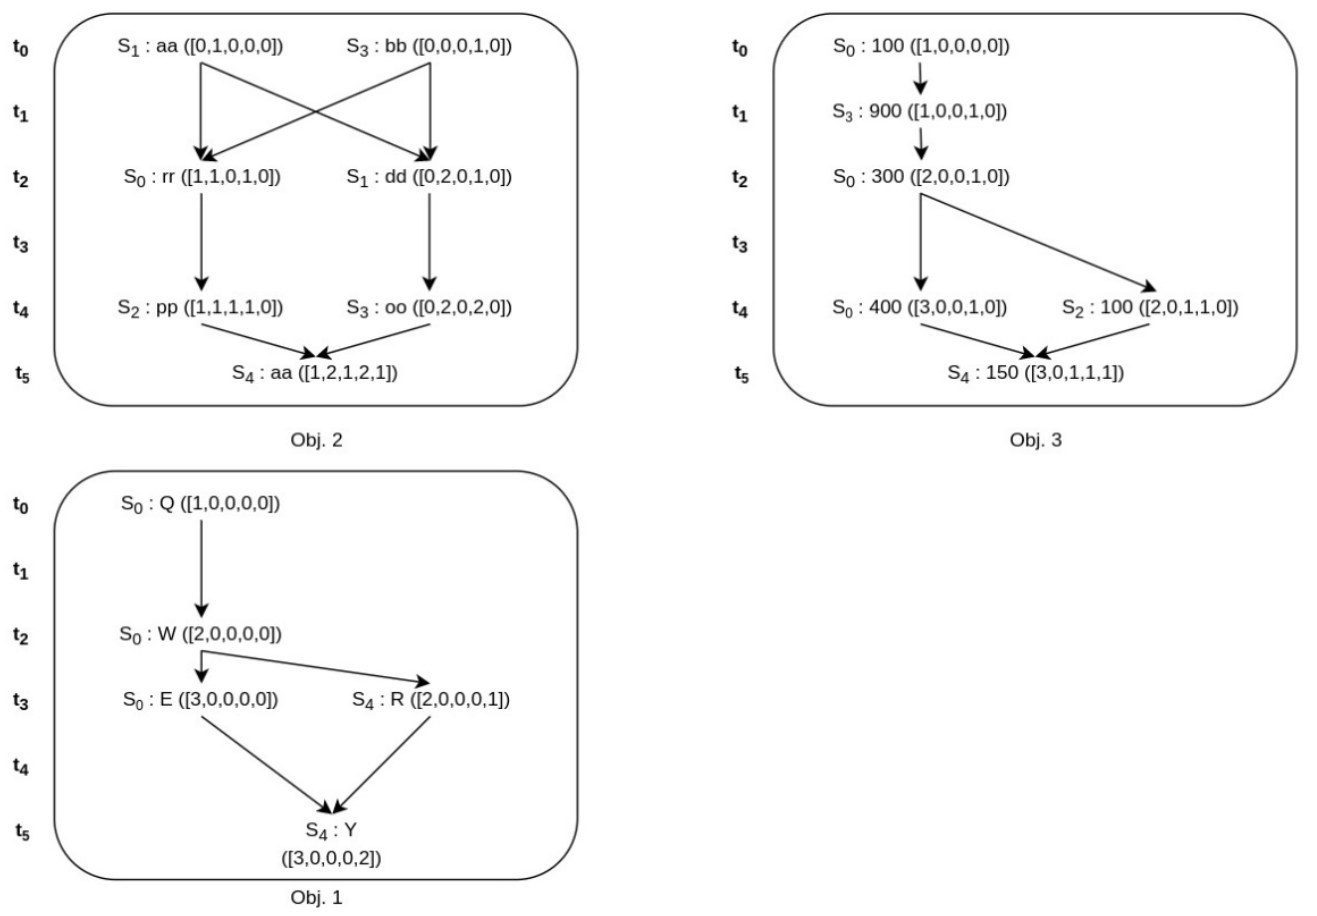
\includegraphics[scale=0.3]{images/6-vs_ex.png}
	\caption{Version Evolution DAGs examples.}
	\label{fig:vc_ex}
\end{figure}

\paragraph{Resolving Get Requests}
When a Dynamo coordinator node receives a get request for a specific key, it collects the latest vector clocks for that value from itself and the top $N-1$ healthy nodes in its preference list for that key. Given a list of value and vector clock pairs, draw the version DAG reconstructed by the coordinator node.

If a get request arrives and we have a DAG with multiple leaves, all vector clocks are returned and the client is responsible for reconciliation (merging the different VCs).

%TODO examples, what is the final value?

%TODO optional exercise, only if in exams and quizzes


\subsubsection{Merkle Trees}

\paragraph{Recap}
Leaves are data blocks and every non-leaf node is labelled with the hash value of its children. Some KeyValue stores use MT to efficiently detect inconsistencies in data between replicas. To compare MT, we first compare the root node - if the values match, the replicas are consistent. Else, compare the next level and follow the tree down until the inconsistent leaf/leaves are identified.

%TODO examples

\paragraph{Comparing Merkle Trees}
Pay special attention to:
\begin{itemize}
    \item If the root hash differs between two MTs but the hash values of the root children are the same in both MTs, it would imply that our hash function produced two different values for the same input values - this is impossible.
    \item It is theoretically possible that two different sets of input values produce the same hash value (parent) because hash functions can have a non-zero probability for hash collisions. This is not an issue with hash functions that are strong enough but it can happen in practice.
\end{itemize}


\subsubsection{Virtual Nodes}

Given a set of nodes, each node with different main memory capacities, and given a number of tokens, find the amount of virtual tokens to give to each node for a fair partition.

\paragraph{Tips}
\begin{itemize}
    \item 1TB = 1024 GB
    \item Capacity per token: total capacity / total number of tokens
    \item It is good practice to give the node with the smallest capacity more than one token (it might be unlucky and get a lot of responsibility). %TODO what
\end{itemize}

%TODO possible exam questions



\subsection{Storage Models}

\subsubsection{Hadoop and HDFS}

%TODO using hadoop exam relevant?

\paragraph{Hadoop Recap}
Hadoop provides a distributed file system and a framework for the analysis and transformation of very large data sets using the MapReduce paradigm. Some components of Hadoop are: HDFS (distributed file system), MapReduce (distributed computation framework), HBase (column-oriented table service), etc. %TODO more on other components?

\paragraph{HDFS Statements}
\begin{itemize}
    \item The HDFS namespace is a hierarchy of files and directories. In contrast with the Object Storage logic model, HDFS is designed to handle a relatively small amount of huge files. A hierarchical file system can therefore be handled efficiently by a single NameNode.
    \item The default size for blocks of a file is either 64 or 128 megabytes - this can be easily changed in the configuration.
    \item No data goes through the NameNode. The client writes data directly to the DataNodes. %TODO ask first?
    \item A DataNode may execute multiple application tasks for different clients concurrently.
    \item The cluster can have thousands of DataNodes and tens of thousands of HDFS clients per cluster.
    \item NameNodes keep the namespace in RAM and an image of such namespace is also persisted in the NameNode file system.
    \item The locations of block replicas are not part of the persistent checkpoint that the NameNode stores in its native file system since they can change over time (re-distribution upon DataNode failure / addition).
    \item If the HDFS block size is 64MB, a 80MB file will be stored on disk as a block of 64MB and 16MB. We don't require extra space since the HDFS blocks are not rounded up to their nominal block size when they're stored (as in disk blocks of traditional file systems). The underlying system stored the two HDFS blocks with their own disk block system (rounded up). We don't require 128MB of physical storage for the 80MB file.
    \item Hardware cost grows linearly as a function of amount of data stored.
    \item NameNode is single point of failure (DataNode failure is handled easily). Run two redundant NameNodes for security (not the same as secondary NameNode which makes startups faster by efficient amount of keeping log and image info). Secondary NameNode does not store data blocks.
\end{itemize}

\paragraph{HDFS Block Size}
The typical HDFS block size is either 64MB or 128MB (compared to 4KB / 4096B in a typical file system - a lot smaller!). Advantages of a large block size are:
\begin{itemize}
    \item Minimize seek cost (much smaller than transfer time). Transfer time is usually at disk transfer rate.
    \item Less client-master interactions - reads/writes on same chunk only require one block location information request from to master. Usual pattern: sequential read/write of large files.
    \item Reduce network overhead since read/write on large chunk (as in typical access pattern) allows for longer persistent TCP connection.
    \item Less metadata stored in master and can be therefore stored in memory.
\end{itemize}

\paragraph{HDFS Properties}
\begin{itemize}
    \item \textbf{Scalability:} Partition files into blocks and distribute them to many servers operating in parallel. Arbitrarily increase storage capacity by simply adding more DataNodes.
    \item \textbf{Durability:} HDFS creates multiple copies of each block (by default 3, on different racks) to minimize the probability of data loss.
    \item \textbf{High sequential read/write performance:} By splitting huge files into blocks and spreading these into multiple machines.
\end{itemize}



\paragraph{Replication Policy}
For each block individually, default is three replicas. One randomly in a node and the other two in a different rack on two separate nodes. Probability of rack failure is much lower of node failure, thus no problem of having 2/3 replicas in same rack.

\paragraph{Write New File}
2-5 are repeated for each block.
\begin{enumerate}
    \item C asks NN to create new file.
    \item C asks NN or DN to host block.
    \item NN replies with a list of DN and locations for block.
    \item C writes to first DN, DN replicates to next and so on.
    \item DNs send ACKs to previous DNs. If all replied, first DN sends ACK to C.
    \item C asks NN to close file and release lock.
    \item DNs check with NN for minimal replication.
    \item NN sends ACK to C.
\end{enumerate}

\paragraph{Read File}
\begin{enumerate}
    \item C requests file from NN.
    \item NN replies with list of blocks and locations of each replica.
    \item C reads each block from closest DN.
\end{enumerate}

\paragraph{Distance Rules}
Network bandwidth is estimated by distance - the shorter the more bandwidth is available. Distance between node and parent = 1, distance between nodes = sum up their distances to closest common ancestor.

To calculate distances, draw a tree where: root = cluster, root kids = datacenters, datacenter kids = racks, rack kids = nodes. From node to node: sum up edges of shortest path. Distance in same node = 0.

\paragraph{HTTP Return Codes}
\begin{itemize}
    \item Successful append operation to a file: 307 and 200
    \item Successful HTTP GET operation for reading and opening a file: 307 and 200
    \item Successful HTTP GET request for listing files: 200
    \item Successful HTTP PUT operation for setting the replication factor: 200
    \item Failed HTTP AUTHENTICATE request: 401
    \item Malformed HTTP GET request for listing files: 400
\end{itemize}

\paragraph{Latency vs. Throughput Block Size}
\begin{itemize}
    \item High latency and high throughput: choose largest possible block size to maximize throughput.
    \item Low latency and normal throughput: choose small(est) block size
\end{itemize}

\subsubsection{Different Storage Models}

\paragraph{Object Storage vs. Block Storage}
\begin{itemize}
    \item Block Storage implements file storage API, whereas Object Storage provides only key-value interface.
    \item Pure Object Storage has a limit on object size, since the object cannot be partitioned across machines. Block Storage does not have this limitation and can split objects into blocks. Therefore, Block Storage can store PB files, whereas Object Storage is limited by the storage capacity of a single node. On the other hand, object storage can store more files than Block Storage.
    \item BS for huge amount of large files, OS for large amount of huge files.
    \item BS allows for block level access, OS can only retrieve entire files.
    \item OS is better for: Netflix movies with many concurrent accesses (movies small enough, simple KV is enough), auto backups of smartphones (written once, rare reads where partial access is not essential)
    \item BS is better for: experimental and simulation data from CERN (large files, store lots of data).
\end{itemize}

%TODO exam questions


\subsection{XML and JSON}

\subsubsection{XML}

%well-formedness checking (enhance tips with encountered examples)

\paragraph{Well-Formedness Additional Tips}
\begin{itemize}
    \item Element names must start with a letter or underscore.
    \item Some escape entities need to be defined like example below for copyright. %TODO which ones, todo escape characters generally
    \item Not allowed to have two attributes with same name. Attribute values have to be quoted.
    \item XML is case-sensitive.
    \item Element names can contain letters, digits, hyphens, underscores, and periods.
    \item Element names cannot contain spaces.
    \item Same tag name is okay
\end{itemize}

\begin{lstlisting}[language=XML]
<!DOCTYPE catalog [
<!ENTITY cright "&#169;">
]>
\end{lstlisting}

\paragraph{Predefined Entities}
\begin{itemize}
    \item \&lt; $<$
    \item \&gt; $>$
    \item \&amp; \&
    \item \&quot; " (okay to not escape)
    \item \&apos; ' (okay to not escape) %TODO right?
\end{itemize}

%TODO namespace practice (ex. 2)


\subsubsection{JSON}

\paragraph{Well-Formedness Additional Tips}
\begin{itemize}
    \item Double quotes
    \item Commas in objects
    \item "type": [["home"]] is okay
    \item "@number": "646 555-4567" is okay
    \item "1phone": 212-3242 needs quotes since there is a dash in number
    \item null with small n
    \item No duplicate keys
    \item Keys are always strings
    \item Using whitespaces and non-ascii characters for key names is allowed although not recommended.
    \item Mixing proper boolean values and strings used as boolean values (ie. "true") is considered a bad practice.
\end{itemize}

%TODO exam questions



\subsection{Wide Column Stores}

%TODO using HBase

\subsubsection{HBase Architecture}

\paragraph{Returning Key Value Pairs}
Given a query for a specific key, the most recent versions of each component are returned (memstore and HFiles). If they have the same timestamp, return both. If one is newer than the other and in the same component and same col., return newest. If they are in different columns, return both (no matter the timestamp)! Multiple values can be returned!

\paragraph{Bloom Filter}
One BF per HFile, used to avoid checking HFiles for a specific key. If no match in BF, don't read file. Key input in various hash functions and then map to array (1 for output value, else 0), for new key, check if sets of 1 is present.

\paragraph{Index}
To avoid scanning HFiles entirely upon get(key) - index helps to skip to HBase block that may hold the key. HBase blocks are not the same as HDFS or FS blocks. They come in 4 varieties: DATA, META, INDEX, and BLOOM. Default size: 64KB and contains whole key/value pairs (block grows to not split a key/value pair).

Build an index exercise: start with first key/value pair in sorted HFile (first pointer). Fill first HBase block by counting bytes of entries (with spill). Second pointer points to first value not fitting in the first HBase block. Index contains: rowID of first key/value pair, key without value, pointer to first key/value pair of block index points to. See Figure \ref{fig:hb_ex} for an example.

\begin{figure}[h]
	\centering
	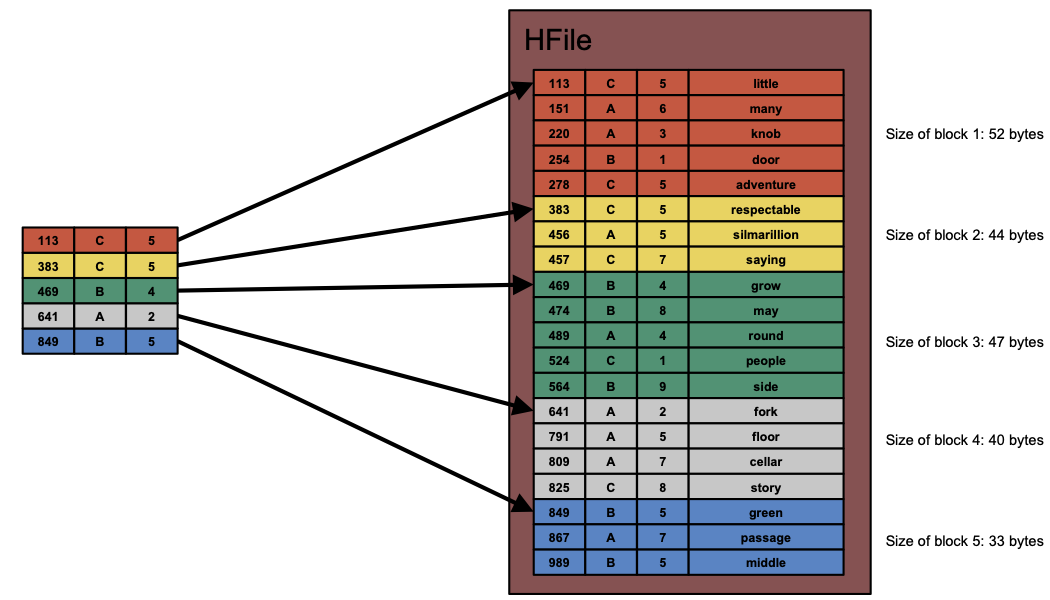
\includegraphics[scale=0.5]{images/6-hb_index.png}
	\caption{Example HBase index.}
	\label{fig:hb_index}
\end{figure}

\paragraph{Schema: Choice of Row Key}
%TODO

\paragraph{Log Structured Merge Trees}
A LSM tree is highly efficient in applications using wide column storage where insertions in memory happen quite often. As opposed to B+-tree which has a time complexity of O(log n) when inserting new elements, n being the total number of elements in the tree, LSM tree has O(1) for inserting, which is a constant cost.

All of the stores are always sorted by key, so no reordering is required to fit new keys in between existing ones. LSM tree promises high write throughput. LSM tree allows random insertion of key-value pairs. 	Flush and compaction do not happen at the same time.

\textbf{Insert:} Writes are inserted in sorted MemStore, which is flushed to disk as a HFile segment if MemStore is too big. Old HFiles are periodically compacted together to save disk space and reduce fragmentation of data.

\textbf{Read:} Lookup key in MemStore. With hash index, search in one or more HFiles (depends on status of compaction).

\textbf{Delete:} Special case of update - store delete marker, use during lookup to skip “deleted” keys. When the pages are rewritten asynchronously, the delete markers and the key they mask are eventually dropped.

\textbf{Exercise:} Writing, reading and deleting key/value pairs. When inserting key/value pairs, sort them in MemStore and note down timestamp (increase also for non-matching keys). Flush MemStore if threshold is reached = sorted HFile on disk. Upon read, check both MemStore and Disk and get latest value. Compact HFiles on disk if threshold reached = sorted HFile, remove duplicate keys with earlier timestamp. Upon delete, keep key/value pair but also store delete marker.

%TODO more on LSM trees

\paragraph{HBase Atomicity Guarantees}
Row-level atomicity.

\paragraph{HBase Replication Functionality}
Setting up a backup HBase cluster in a separate datacenter to be synced with the current cluster. NOT the management of row replicas on many RegionServers.

\paragraph{HBase vs. RDBMS}
\begin{itemize}
    \item HBase for: Data schema is difficult to determine in advance, or changes frequently and most of the data is sparse.
    \item RDBMS for: Dense and highly-structured data and Database consistency must always be maintained.
\end{itemize}

\paragraph{Write-Ahead Log (WAL)}
Without the WAL, in order to keep guaranteeing durability every write operation would require sorting an HFile.



\subsection{Validation}

\subsubsection{XML Information Set}

\paragraph{Recap}
XML "Information Set" provides an abstract representation of an XML document — it can be thought of as a set of rules on how one would draw an XML document on a whiteboard. An XML document has an information set if it is well-formed and satisfies the namespace constraints. There is no requirement for an XML document to be valid in order to have an information set. An information set can contain up to eleven different types of information items, e.g., the document information item (always present), element information items, attribute information item, etc. Information sets can be drawn as trees.

\textbf{Example 1:} Tree can contain: document information item, elements, character information items, and attributes. See tree in \ref{fig:xml_tree1}.

\begin{lstlisting}[language=XML]
<Burger>
    <Bun>
        <Pickles/>
        <Cheese origin="Switzerland" />
        <Patty/>
    </Bun>
</Burger>
\end{lstlisting}

\begin{figure}[h]
	\centering
	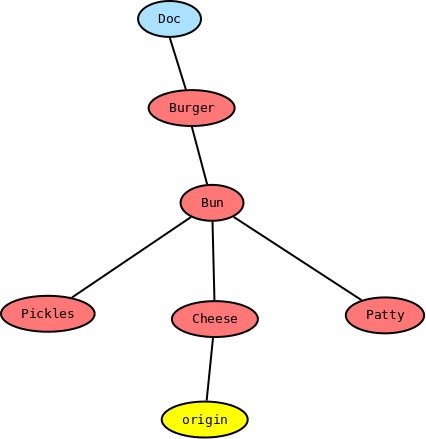
\includegraphics[scale=0.3]{images/6-xml_tree1.png}
	\caption{Example 1 XML tree.}
	\label{fig:xml_tree1}
\end{figure}

\textbf{Example 2:} Tree can contain: document information item, elements, character information items, and attributes. See tree in \ref{fig:xml_tree2}.

\begin{lstlisting}[language=XML]
<catalog>
   <!-- A list of books -->
   <book id='bk101'>
      <author>Gambardella, Matthew</author>
      <title>XML Developer's Guide</title>
      <genre>Computer</genre>
      <price>44.95</price>
      <publish_date version='hard' version2='soft'>2000-10-01</publish_date>
   </book>
</catalog>
\end{lstlisting}

\begin{figure}[h]
	\centering
	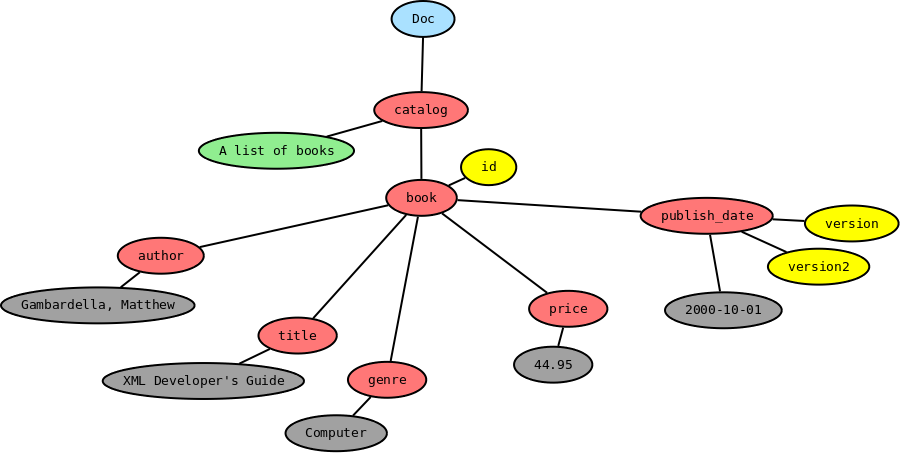
\includegraphics[scale=0.3]{images/6-xml_tree2}
	\caption{Example 2 XML tree.}
	\label{fig:xml_tree2}
\end{figure}

\textbf{Example 3:} Tree can contain: document information item, elements, character information items, namespace items and attributes. See tree in \ref{fig:xml_tree3}.

\begin{lstlisting}[language=XML]
<?xml version="1.0"?>
<!DOCTYPE eth>
<eth xmlns="http://www.ethz.ch" xmlns:ethdb="http://www.dbis.ethz.ch" date="11.11.2006" ethdb:date="12.11.2006">
   <date>16.11.2017</date>
   <president since="2015">Prof. Dr. Lino Guzzella</president>
   <ethdb:Rektor>Prof. Dr. Sarah M. Springman</ethdb:Rektor>
</eth>
\end{lstlisting}

\begin{figure}[h]
	\centering
	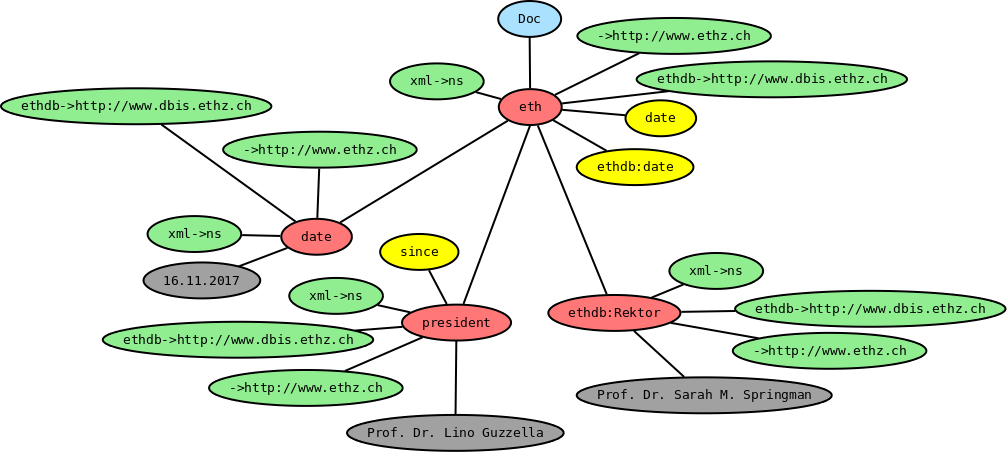
\includegraphics[scale=0.3]{images/6-xml_tree3}
	\caption{Example 3 XML tree.}
	\label{fig:xml_tree3}
\end{figure}

%TODO more on what items mean


\subsubsection{XML Schema}

\paragraph{Recap}
An XML Schema describes the structure of an XML document. The purpose of an XML Schema is to define the legal building blocks of an XML document: the elements and attributes that can appear in a document, the number of (and order of) child elements, data types for elements and attributes, default and fixed values for elements and attributes.

\paragraph{Validation: Document Matches Schema}
%TODO examples

\paragraph{Provide Schema}
%TODO




\subsubsection{JSON Schema}

\paragraph{Recap}
JSON Schema is a vocabulary that allows you to annotate and validate JSON documents. It is used to: describe your existing data format(s), provide clear human- and machine- readable documentation, validate data, i.e., automated testing, ensuring quality of client submitted data.

%TODO



\subsubsection{Document Validation}

\paragraph{Document Type and Validation}
\begin{itemize}
    \item \textbf{XML:} XML Schema, DTD, Schematron, RelaxNG, or not validated at all
    \item \textbf{JSON:} JSON Schema, JSound, Kwalify, or not validated at all
    \item \textbf{Protocol Buffers:} Protocol buffer schema language, it always has to be validated
    \item \textbf{XHTML:} XHTML XML Schema
\end{itemize}



\subsubsection{Dremel}

\paragraph{Recap}
Dremel is a query system developed at Google for deriving data stored in a nested data format such as XML, JSON, or Google Protocol Buffers into column storage, where it can be analyzed faster.

\paragraph{Conversion Algorithm}
Convert nested data format with an associated schema (e.g. Google Protocol Buffer document and schema) into column storage.

%TODO look at example, same record attention, practice, when to NULL



\paragraph{Statements}
\begin{itemize}
    \item False: Column storage takes up more disk space than nested data to allow for faster read-only operations. %TODO ?
    \item Dremel does not use standard SQL as its query language.
    \item False : After converting to column storage using the Dremel method, we can use this representation to speed up writes to the original data source. %TODO ?
    \item Column storage is faster than row storage at performing projections.
\end{itemize}






\subsection{MapReduce}


%TODO MapReduce Java API



\subsubsection{Reverse Engineering}
%TODO MR to SQL
%TODO python and SQL!!!

\subsubsection{True/False, Facts}

\paragraph{True}
\begin{itemize}
    \item MapReduce splits might not correspond to HDFS blocks. Since splits respects logical record boundaries, they might contain data from multiple HDFS blocks.
    \item One single Reducer is applied to all values associated with the same key. This is the principle behind partitioning: one Reducer is responsible for all values associated with a particular key.
    \item Multiple Reducers can be assigned pairs with the same value. Values are not relevant in partitioning.
\end{itemize}

\paragraph{False}
\begin{itemize}
    \item Each mapper must generate the same number of key/value pairs as its input had. Why: For each input pair, the mapper can emit zero, one, or several key/value pairs.
    \item The TaskTracker is responsible for scheduling mappers and reducers and make sure all nodes are correctly running. Why: The JobTracker is responsible for this.
    \item The input key/value pairs of mappers are sorted by the key. Why: mapper input is not sorted.
    \item In Hadoop MapReduce, the key-value pairs a Reducer outputs must be of the same type as its input pairs. Why: Reducer's input and output pairs might have different types.
\end{itemize}

\paragraph{Benefits of Combine Function}
\begin{itemize}
    \item Decrease memory requirements on Reducers (but not in mappers)
    \item Decrease the overall communication volume
    \item Does not decrease mapper computation time
\end{itemize}

\paragraph{Load Balancing}
Requires prior knowledge about the distribution of keys - good partitioning function. Not automatic. %TODO partitioning function examples

\paragraph{Inefficiency}
MR is always inefficient if: reducers get a lot of data with a small amount of possible keys.



\subsection{YARN and Spark}

\subsubsection{YARN}

\paragraph{Issues Addressed}
\begin{itemize}
    \item \textbf{Scalability:} MapReduce has limited scalability, while YARN can scale to 10,000 nodes.
    \item \textbf{Rigidity:} MapReduce v1 only supports MapReduce specific jobs. There is a need, however, for scheduling non-MapReduce workloads. For instance, we would like the ability to share cluster with MPI, graph processing, and any user code.
    \item \textbf{Resource Utilization:} in MapReduce v1, the reducers wait on the mappers to finish (and vice-versa), leaving large fractions of time when either the reducers or the mappers are idle. Ideally all resources should be used at any given time.
    \item \textbf{Flexibility:} mapper and reducer roles are decided at configuration time, and cannot be reconfigured.
\end{itemize}


\subsubsection{Schedulers}

\paragraph{FIFO}
Application in queue, run in order of arrival. No time guarantees.

\paragraph{Fair Scheduler}
All applications have same priority and resources are fairly distributed. Resources are dynamically balances between running jobs. New job - find new balance. If preemption is enabled, reclaiming of resources is instant (termination of running jobs possible) - else wait until resources freed up.

\paragraph{Capacity Scheduler}
Each user has certain minimum capacity guarantees. Resources are allocated over a set of predetermined queues. Each queue gets only a fraction of the cluster resources. As a result, each queue has a minimum guaranteed resource allocation. Capacity Schedulers feature two different metrics for assigning resources: SFS and IFS. %TODO formulas?

\paragraph{Compute SFS}
Given resources (memory, cores, amount of nodes) and hierarchical queue config, compute SFS.
\begin{enumerate}
    \item Calculate total capacity (total amount of memory and cores).
    \item SFS for each queue: first level simply demand / 100, second level parent result times (demand / 100).
    \item For each node (!), result times resources.
\end{enumerate}

\paragraph{CS vs. FS}
\begin{itemize}
    \item In CS and with no queue elasticity, applications submitted to a queue that does not have enough resources will be rejected.
    \item In FS, always count with the full resources.
\end{itemize}

\paragraph{DFS Exercise}
%TODO, what about queues? TODO!!! on paper




\subsubsection{Spark Architecture}

%TODO setting up spark in azure?

%RDD coding stuff, parallelize stuff, partitioning (also in moodle), bunch of lambda functions

%spark UI

%TODO RM, AM, NM responsibilities







\subsection{Spark Dataframes and SparkSQL}

%TODOOOOO







\subsection{Document Stores (MongoDB)}


\paragraph{Normalized Data in DS}
References can be used for data normalization. In Figure \ref{fig:mdb_norm}, instead of storing contact and access as nested objects in the user document, new documents with a foreign key are created and referenced in the original. 

Different relationships between data can be represented by references and embedded documents. %TODO embedded documents?

\begin{figure}[h]
	\centering
	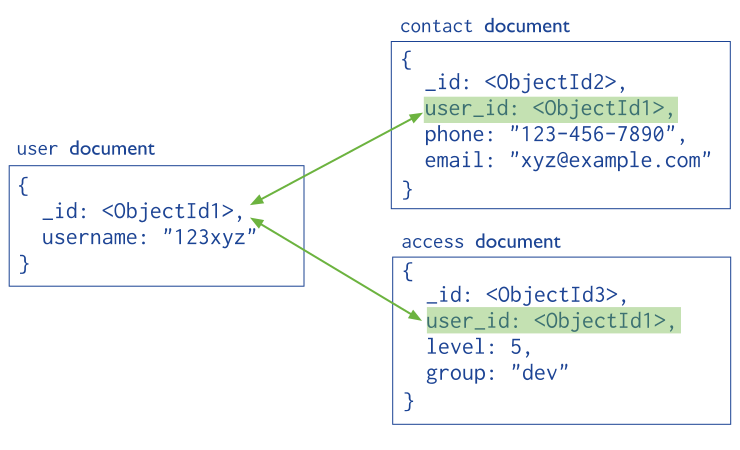
\includegraphics[scale=0.3]{images/6-mdb_norm.png}
	\caption{How to normalize data in MongoDB.}
	\label{fig:mdb_norm}
\end{figure}

\paragraph{DS vs. KVS}
Document-oriented databases are inherently a subclass of the key-value store. The difference lies in the way the data is processed: in a key-value store, the data is considered to be inherently opaque to the database, whereas a document-oriented system relies on an internal structure of the documents in order to extract metadata that the database engine uses for further optimization. Although the difference is often mostly in tools of the systems, conceptually the document-store is designed to offer a richer experience with modern programming techniques.

\paragraph{Data Model to Document Mapping}
%TODO

\paragraph{Writing MongoDB}
%TODO? projection dont forget to remove id if not wanted, what about "?
%TODO 24h question
%TODO operators with $
%value of _id cannot be changed with queries?
%array with find also counts (moodle)
%Scalars (non-array elements) in documents must match each clause of a query’s criteria. However, if a document’s "x" field is an array, the document matches if there is an element of "x" that matches each part of the criteria but each query clause can match a different array element.

\paragraph{MongoDB Indices}
%TODO
%where queries
%Only one field in an index entry can be from an array. This is to avoid the explosive number of index entries you’d get from multiple multikey indexes: every possible pair of elements would have to be indexed, causing indexes to be n*m entries per document.
%arrays

\paragraph{Padding}
The padding factor is the amount of extra space MongoDB leaves around new documents to give them room to grow. When MongoDB has to move a document, it bumps the collection’s padding factor. You can see the padding factor by running db.coll.stats().

\paragraph{Cursor}
Almost every method on a cursor object returns the cursor itself so that you can chain options in any order. %TODO more on cursors

\paragraph{Type Comparison Order}
%TODO 
\url{https://docs.mongodb.com/manual/reference/bson-type-comparison-order/}



\subsection{Rumble}


\paragraph{Idempotent Queries}
Any JSON document is also a JSONiq query. Running a JSON document as a query just outputs itself. This also works the other way round: if your query outputs an object or an array, you can use it as a JSON document.

%TODO programming (install first...)

% we need to check all elements in array - another for
%count and order by $c clause

%importing two json files has to be separate, no comma notation





\subsection{Graph Databases and Neo4j}


%TODO cypher querying........

\begin{itemize}
    \item In Neo4j, relationships can be traversed in either direction with the same cost.
    \item The starting points of our graph queries are called bound nodes.
    \item In Neo4j an edge stores pointers to all the edges of both the source and the target nodes, using double-linked lists.
    \item With index free adjacency every record stores a pointer to the relationships connected to that node, making the lookup of relationship in costant time.
    \item B-Tree index lookups on a relational database with n elements : O(log n)
    \item Doing an m step/hop traversal on a graph with n elements and use index free adjacency: O(m)
    \item Traverse a network of m steps/hops with n elements using index lookups : O(m*logn)
    \item Looking up immediate relationships in a graph database with index free adjacency : O(1)
    \item Neo4j transactions are ACID-compliant, committing data to disk in Neo4j uses a Write Ahead Log
    \item Neo4j (labelled property graph) and RDF (triple stores)
    \item Neo4j uses a query by example paradigm, while SPARQL follows a declarative query paradigm similar to SQL
    \item In RDF a property can also be the source or the target of another triple
    \item 
\end{itemize}



\subsection{OLAP and Cubes, Data Warehousing}


%TODO SQL shit

Given a fact table with m dimensions and n different possible values for each dimension and assuming that it has no duplicate rows or missing values, the amount of rows in the fact table is: $n^m$, this represents all combinations between all possible values for all dimensions.

Creating a view for the full data cube (adding rows with Nulls for slice aggregations) out of this fact table gives us $(n+1)^m$ rows (as we now have the possibility of aggregating over a dimension, and we represent this by using a Null value for that dimension. Therefore, it's as if we have a new "possible value" for our dimensions, this value being Null).